\input{"../../../preamble"}

\begin{document}

\title{CSC263-Notes-01-19-2015}

\input{"../csc263-header"}
\rhead{January 19, 2015}

\reversemarginpar
\mpreadings

\noindent Part III (Intro), Sections 12.1, 12.2, 12.3

\mpselftest

\noindent Exercises 12.2-3, 12.3-1

\section*{Lecture 05}

\subsection*{Dictionaries}

\noindent keys: 5 7 2 0 20 4 9 \\

\noindent \textbf{Objects}:= Sets $s$ where each element $x$ has field \texttt{x.key} - some totally 
	ordered value. Keys are distinct. \\

\noindent \textbf{Operations}: 
\begin{itemize}
	\item \texttt{search(S,k)}: return $x \in S$ s.t. $x.key = k$, or NIL if no such $x$
	\item \texttt{delete(S,x)}: remove $x$ from $S$ (given element $x \in S$ not just $x.key$ or the values in the element) \\
		\begin{tabular}{l @{: } p{15cm}}
			Q & Why not \texttt{delete(S,k)?} \\
			A & Achieved with \texttt{delete(S,search(S,k))}, separates ``searching phase'' from ``deletion'' phase, making it possible to analyse each one seperately
		\end{tabular} \\
		Notice that \texttt{delete} assumes that we not only know the element $x$'s values but that we have a pointer to the actual element $x$ in the data structure.
	\item \texttt{insert(S,x)}: insert $x$ in $S$; if some $y \in S$ has $y.key = x.key$, replace $y$ by $x$
\end{itemize}

\noindent \begin{tabular}{| l | l | l | l | l | l | l |}
	\hline 5 & 7 & 2 & 8 & 20 & 4 & 9 \\ \hline
\end{tabular} size[7] \\
Complexity of \texttt{search}, \texttt{insert} for unsorted array $\in \Theta(n)$, \texttt{delete} 
	$\in \Theta(1)$\\

\noindent \begin{tabular}{| l | l | l | l | l | l | l |}
	\hline 0 & 2 & 4 & 5 & 7 & 9 & 30 \\ \hline
\end{tabular} size[7] \\
Complexity of \texttt{search} (binary) $\in \Theta(\log n)$, \texttt{insert}, \texttt{delete} $\in \Theta(n)$ \\


\noindent head $\rightarrow 5 \leftrightarrow 7 \leftrightarrow 2 \leftrightarrow 0 \leftrightarrow 20 \leftrightarrow 4 \leftrightarrow 9$ \\
Complexity of \texttt{search}, \texttt{insert} $\in \Theta(n)$, \texttt{delete} $\in \Theta(1)$ \\

\noindent head $\rightarrow 0 \leftrightarrow 2 \leftrightarrow 4 \leftrightarrow 5 \leftrightarrow 7 \leftrightarrow 9 \leftrightarrow 20$ \\
Complexity of \texttt{search}, \texttt{insert} $\in \Theta(n)$, \texttt{delete} $\in \Theta(1)$ \\


\begin{center}
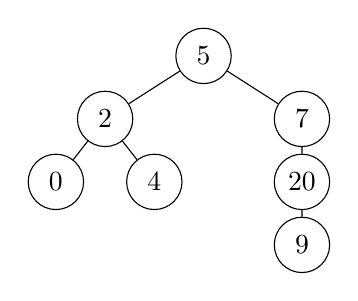
\begin{tikzpicture}[every node/.style={circle,draw,minimum size=2em,inner sep=1},
	baseline={(current bounding box.center)},
	level/.style={level distance=8mm,
	sibling distance=25mm/#1}]
\node {5} 
child {node {2}
	child {node {0}}
	child {node {4}}
	}
child {node {7}
	child {node {20}
		child {node {9}}
		}
	};
\end{tikzpicture}
\end{center}
Complexity of \texttt{search} $\in O(h)$

\subsection*{Summary}

\begin{tabular}{l l l l}
	Data Structure & \texttt{search} & \texttt{insert} & \texttt{delete} \\
	unsorted array & $n$ & $n$ & $1$ \\
	sorted array & $\log n$ & $n$ & $n$ \\
	unsorted singly-linked list & $n$ & $n$ & $n$ \\
	unsorted doubly-linked list & $n$ & $n$ & $1$ \\
	sorted doubly-linked list & $n$ & $n$ & $1$ \\
	binary search tree & $n$ & $n$ & $n$ \\
	balanced search tree & $\log n$ & $\log n$ & $\log n$ \\
	direct-access table(+) & 1 & 1 & 1 \\
	hash table & $n$ & $n$ & $n$ \\
\end{tabular}

\noindent (+) $\rightarrow$ all have space complexity $O(n)$ except direct-access tables, which require space equal to size of universe, e.g., if keys are 32-bit integers, a direct-access table requires space $\Omega(2^{32}$.


\end{document}